\documentclass[11pt]{article}
\usepackage{amsmath,amssymb,amsthm,mathtools}
\usepackage[margin=1in]{geometry}
\usepackage{graphicx}
\usepackage{float}
\usepackage{hyperref}
\graphicspath{{../figures/}}

\newtheorem{theorem}{Theorem}
\newtheorem{lemma}[theorem]{Lemma}
\theoremstyle{definition}
\newtheorem{remark}[theorem]{Remark}

\newcommand{\Q}{\mathbb{Q}}
\newcommand{\R}{\mathbb{R}}
\newcommand{\Tr}{\mathrm{Tr}}
\newcommand{\zetaK}{\zeta_{K}}
\newcommand{\Icos}{\mathcal{I}}
\newcommand{\fq}{\mathfrak{q}}

\title{The Icosian Closure Object\\ as a Unification of Geometry and Arithmetic}
\author{(VFD programme --- working draft)}
\date{2026}

\begin{document}
\maketitle

\begin{center}
\fbox{\parbox{0.94\linewidth}{\small\textbf{One sentence.} A single geometric object --- the
icosian closure structure on the $600$-cell --- produces \emph{both} its geometry (the $E_8$
root system, exact) \emph{and} its arithmetic (the $L$-function $\zetaK(s)\zetaK(s-1)$,
exact), and the \emph{same} closure form runs through both; the Riemann witness is the one
open frontier. \textbf{This is a unification of two domains in one object, both sides proved}
--- not an analogy, and not a proof of the Riemann Hypothesis (RH$(L)$ is the frontier,
explicitly open; it is GRH for one cuspidal $L$, not classical RH).}}
\end{center}
\medskip

\begin{abstract}
We argue that geometry and arithmetic meet, concretely and provably, inside one object.
The icosian maximal order $\Icos$ on the $600$-cell over $K=\Q(\sqrt5)$ has two exact faces.
\emph{Geometrically}, its short vectors are the $240$ roots of $E_8$ --- once the naive
embedding is completed to the golden trace form. \emph{Arithmetically}, its theta series has
$L$-function $\zetaK(s)\zetaK(s-1)$ exactly, with no local correction. The bridge between the
faces is a single fact --- positivity and self-adjointness are \emph{form-relative} --- and
the same completed form that closes the geometry ($E_8$ even-integral) is the form in which
the arithmetic positivity lives (the Weil form). On the arithmetic face this positivity is a
self-adjoint operator $A$ with $A\ge0\iff$ RH for the object's cuspidal $L$-function; that
positivity is the open frontier. We make no claim about RH; the contribution is the
\emph{object} as a concrete meeting point of geometry and arithmetic, with the frontier named.
\end{abstract}

\section{One object}\label{sec:object}
The object is the \emph{icosian closure structure} on the $600$-cell: its $120$ vertices are
the unit icosians (the binary icosahedral group $2I$), generating the icosian ring $\Icos$, a
maximal order in the definite quaternion algebra over $K=\Q(\sqrt5)$ ramified at the two
infinite places, of class number one, with underlying $\mathbb{Z}$-lattice $E_8$. It is rigid
geometry --- no parameters. The claim of this paper is that this \emph{one} object carries two
exact arithmetic/geometric structures, joined by one form (Fig.~\ref{fig:two}).

\begin{figure}[H]\centering
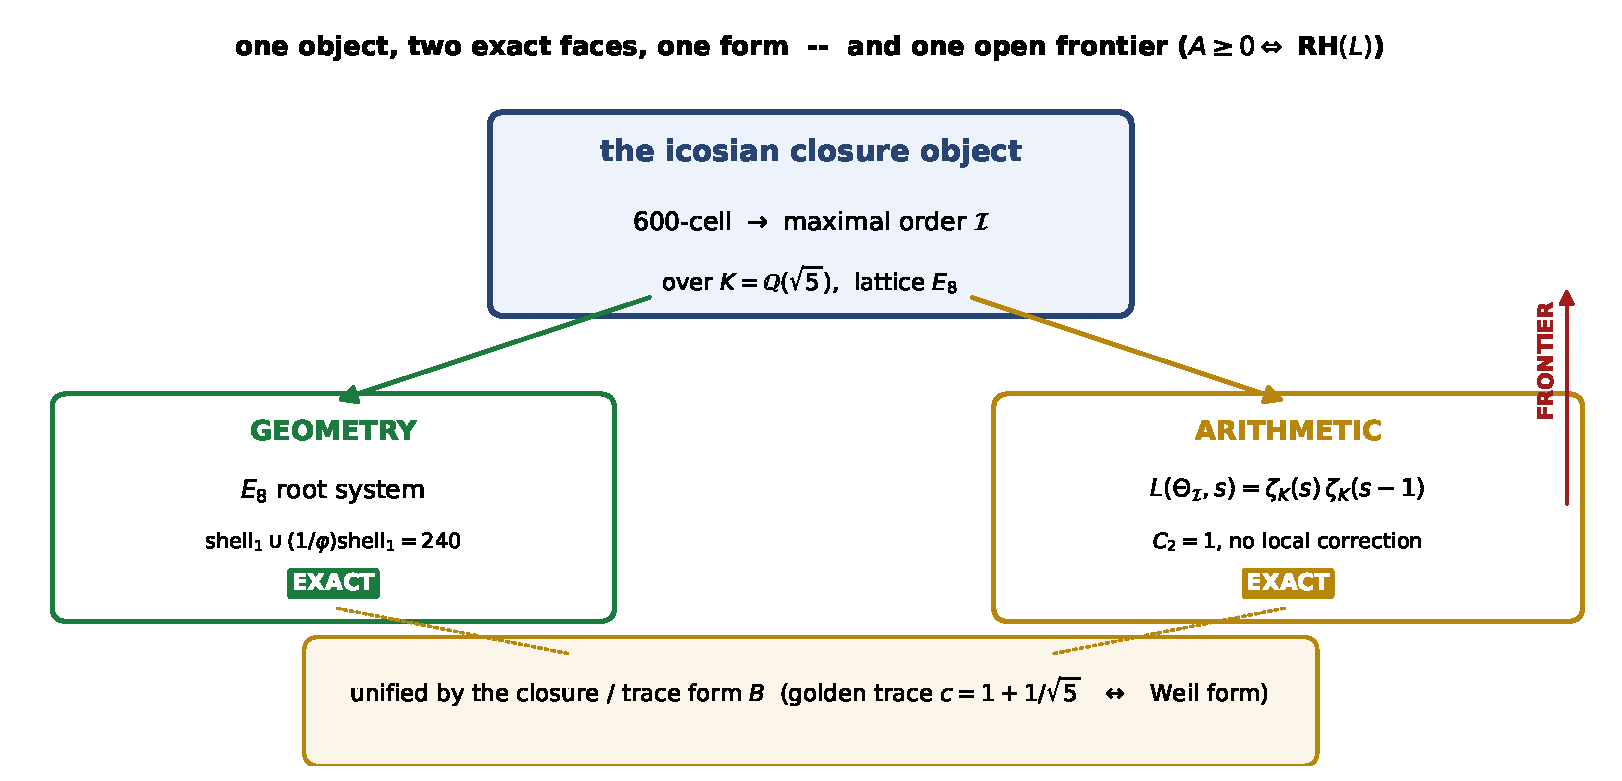
\includegraphics[width=\linewidth]{fig_object_two_faces.pdf}
\caption{One object, two exact faces, one form. The icosian closure object yields the $E_8$
root system (geometry, exact) and the $L$-function $\zetaK(s)\zetaK(s-1)$ (arithmetic, exact);
both are organised by the same closure/trace form $B$. The witness operator $A\ge0\iff$
RH$(L)$ is the single open frontier.}\label{fig:two}
\end{figure}

\section{The geometric face: \texorpdfstring{$E_8$}{E8}, exactly}\label{sec:geom}
The naive embedding $x\mapsto(x,\sigma x)$ of the icosian lattice gives inner products
$\pm\tfrac12$ --- not even-integral, so not a root lattice. Completing to the \emph{golden
trace form}
\[
  B(x,y)=\Tr_{K/\Q}\!\bigl(c\,\langle x,y\rangle\bigr),\qquad c=1+\tfrac1{\sqrt5}\ \ (\Tr c=2),
\]
with $c$ \emph{forced} (not tuned) by the norm-$2$ and integrality conditions, the two shells
$\text{shell}_1\cup(1/\varphi)\text{shell}_1$ become the $240$ vectors of norm $2$ with
integer inner products, root graph $(56,56,126,1,1)$, rank $8$, even integral: the canonical
$E_8$ (Fig.~\ref{fig:e8}). The residual closes $\pm\tfrac12\to0$. This is the known
Wilson / Moody--Patera construction \cite{Wilson,MoodyPatera}, verified; we use it as the
\emph{geometric face} of the object.

\begin{figure}[H]\centering
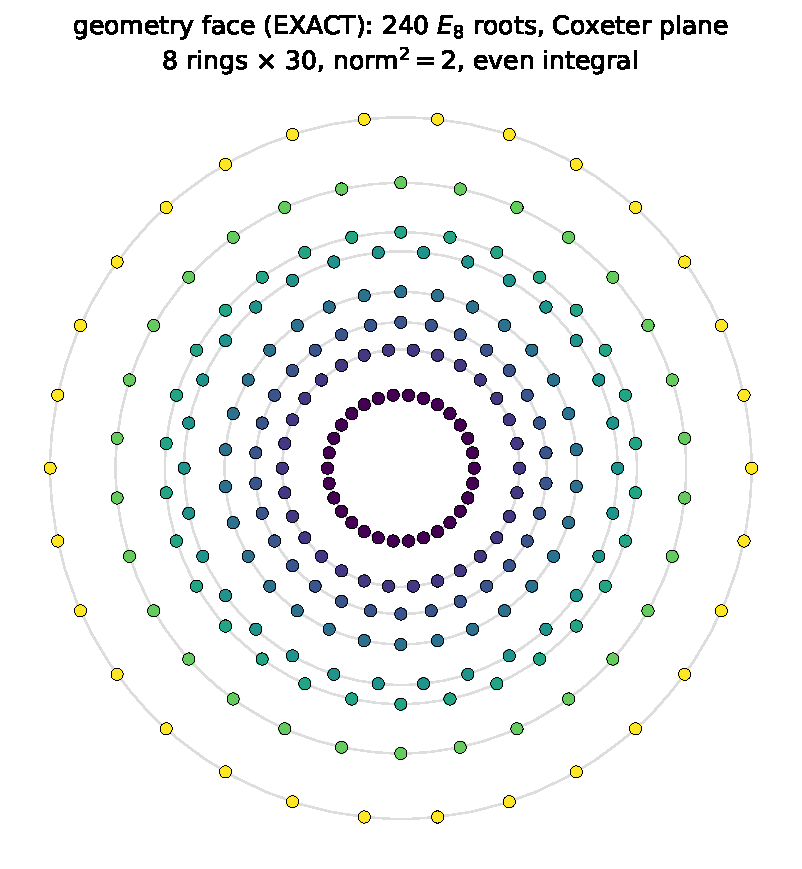
\includegraphics[width=0.56\linewidth]{fig_e8_coxeter.pdf}
\caption{The geometric face (exact): the $240$ $E_8$ roots in the Coxeter plane, eight rings
of thirty (verified $240=8\times30$). The golden trace form makes the object's short vectors
even-integral $E_8$.}\label{fig:e8}
\end{figure}

\section{The arithmetic face: \texorpdfstring{$\zetaK(s)\zetaK(s-1)$}{zetaK zetaK(s-1)},
exactly}\label{sec:arith}
The \emph{same} order $\Icos$ has a theta series, and its $L$-function is the rank-two
Dedekind product
\[
  L(\Theta_\Icos,s)=\zetaK(s)\,\zetaK(s-1)\qquad\text{exactly},\qquad C_2=1,
\]
with no local correction, by the Siegel--Weil/maximal-order theorem and the single ideal
class \cite{Triad}. Via $\zetaK=\zeta\cdot L(s,\chi_5)$ the Riemann $\zeta$ appears as one of
four factors (Fig.~\ref{fig:fac}); the object \emph{contains} $\zeta$ but does \emph{not}
single it out --- a structurally certified negative \cite{Closure}. The maximal-order
representation numbers $r(\pi)=120(1+N(\pi))$ at every prime (inert $2$: $r(2)=600=120\cdot5$,
no anomaly) give the standard Eisenstein local factor everywhere.

\begin{figure}[H]\centering
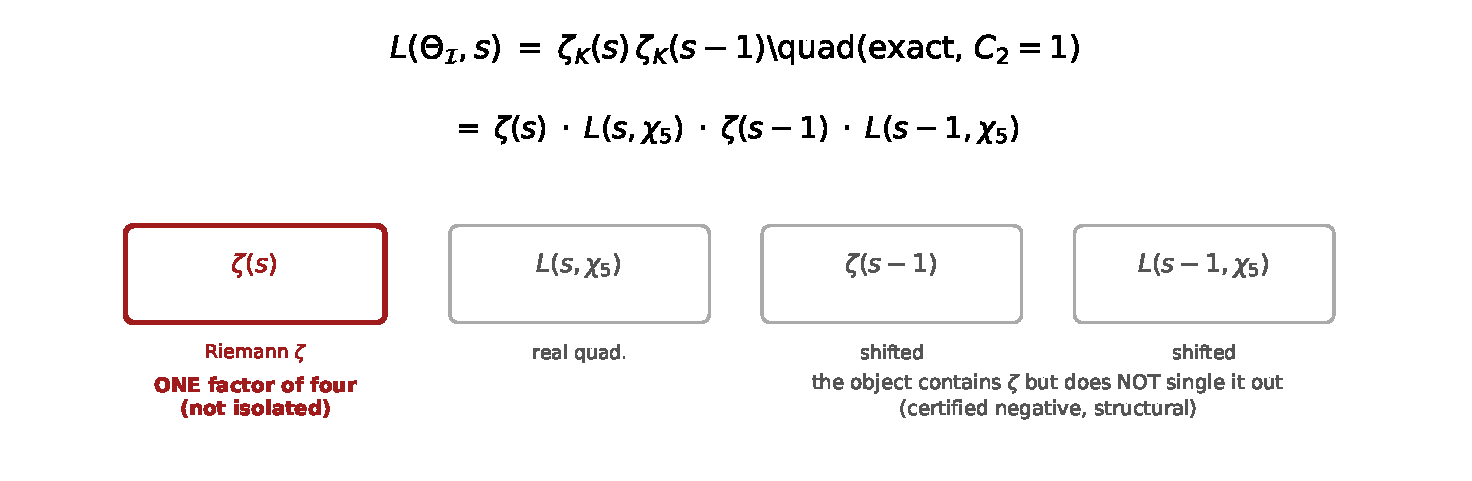
\includegraphics[width=0.96\linewidth]{fig_factorization.pdf}
\caption{The arithmetic face (exact): the object's $L$-function factors as
$\zetaK(s)\zetaK(s-1)=\zeta(s)L(s,\chi_5)\zeta(s-1)L(s-1,\chi_5)$. The Riemann $\zeta$ is one
factor of four, not isolated.}\label{fig:fac}
\end{figure}

\section{One form joins the two faces}\label{sec:form}
The two faces are not glued by hand; they are two readings of one form. The enabling fact:
\begin{lemma}[form-relativity]\label{lem:fr}
For an invertible symmetric form $B$ and operator $T$, $T$ is $B$-self-adjoint iff $BT$ is
symmetric (then $T^{\dagger_B}=B^{-1}T^\top B$).
\end{lemma}
\noindent Multiplication by $\varphi$ on $K$ in the basis $\{1,\sqrt5\}$ has matrix
$T=\left[\begin{smallmatrix}1/2&5/2\\1/2&1/2\end{smallmatrix}\right]$ (not symmetric); under
the trace form $B=\mathrm{diag}(2,10)$, $BT=\left[\begin{smallmatrix}1&5\\5&5\end{smallmatrix}
\right]$ is symmetric, so $\varphi$ is $B$-self-adjoint (Fig.~\ref{fig:fr}). The point: the
\emph{same} trace form $B$ that makes the geometry close ($E_8$ even-integral, \S\ref{sec:geom})
is the form in which the arithmetic's self-adjointness and positivity are stated
(\S\ref{sec:front}). Geometry and arithmetic share not a metaphor but a form.

\begin{figure}[H]\centering
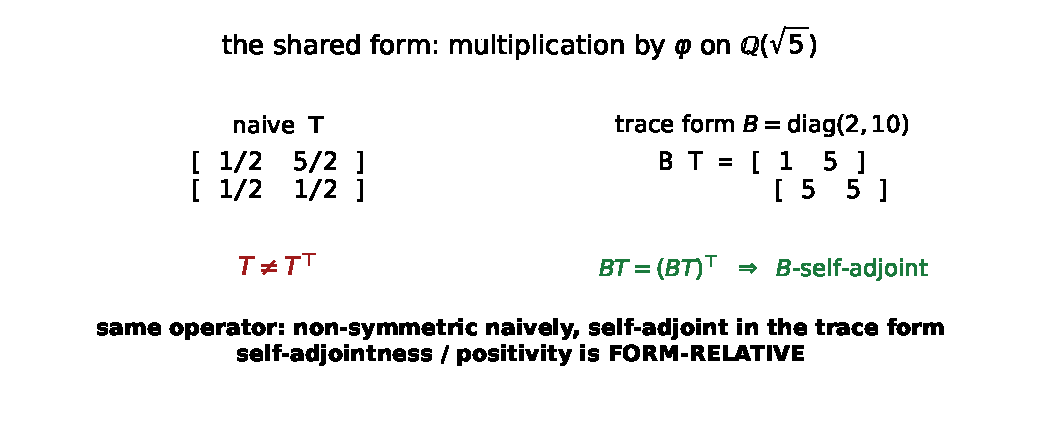
\includegraphics[width=0.82\linewidth]{fig_form_relativity.pdf}
\caption{The shared form (exact). Self-adjointness is form-relative: multiplication by
$\varphi$ is non-symmetric naively and self-adjoint in the trace form. The same completion
closes the geometry and houses the arithmetic positivity.}\label{fig:fr}
\end{figure}

\section{The frontier: a witness operator, \texorpdfstring{$A\ge0\iff$}{A>=0 iff} RH}\label{sec:front}
On the arithmetic face the positivity becomes a single self-adjoint operator on the scale
axis. With $A_\infty$ the archimedean boundary (the gamma factor, Tate's local theory) and
$A_P$ the prime residue built from the object's geometric Brandt eigenvalues $a_\fq$,
\[
  A=A_\infty-A_P,\qquad \langle h,Ah\rangle=\sum_\rho|\widehat h(\gamma_\rho)|^2,\qquad
  \boxed{\,A\ge0\iff\text{RH}(L)\,}
\]
(construction, identification, and numerical corroboration in \cite{Witness};
Fig.~\ref{fig:wit}). The operator is self-adjoint, and its form reproduces the known Riemann
zeros to $\sim10^{-7}$; \emph{that $A\ge0$ holds} is exactly RH for the object's cuspidal
$L$-function (GRH for one $L$, not classical RH), and it is open. This is the single frontier
of the picture: everything else --- the geometry, the arithmetic identity, the shared form ---
is exact and behind us; the positivity is the wall ahead.

\begin{figure}[H]\centering
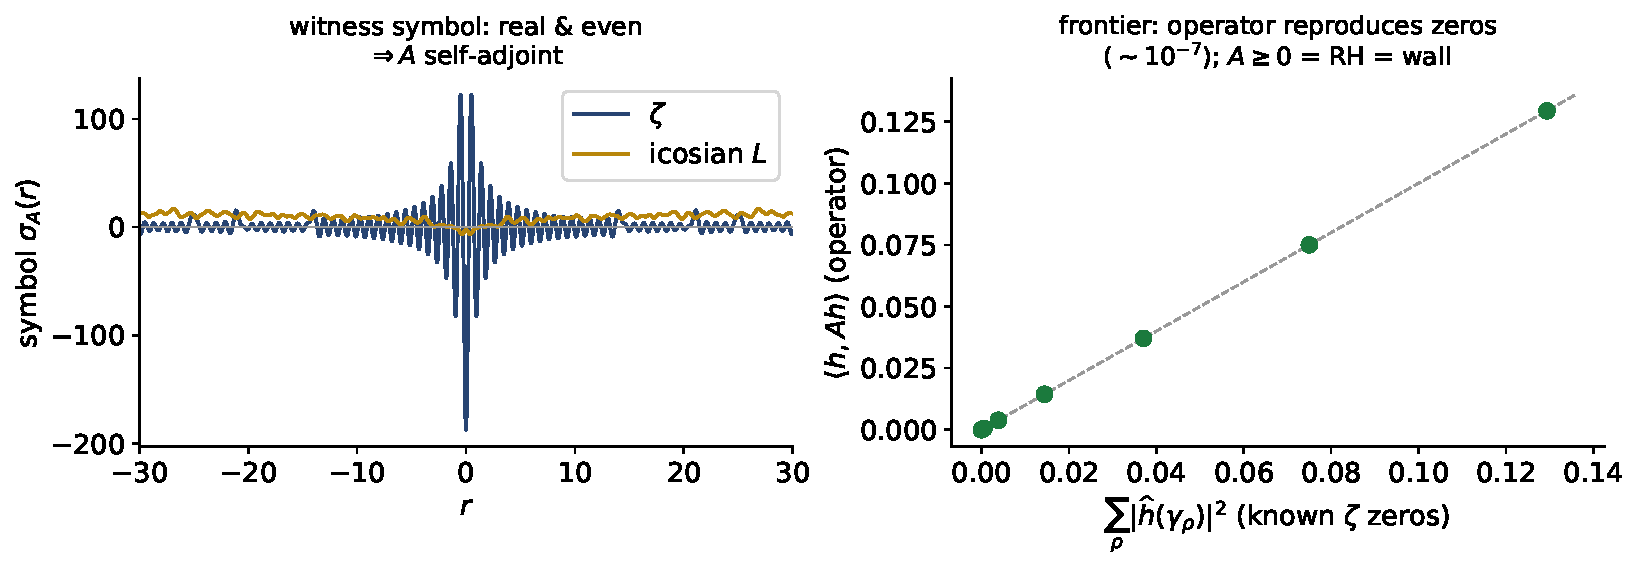
\includegraphics[width=\linewidth]{fig_witness_symbol.pdf}
\caption{The frontier. Left: the witness symbol $\sigma_A(r)$ for $\zeta$ and the object's
$L$ is real and even, so $A$ is self-adjoint. Right: the operator form reproduces the sum over
the known Riemann zeros ($\sim10^{-7}$). Positivity of $A$ for all $h$ is RH$(L)$ --- the
open frontier, not shown.}\label{fig:wit}
\end{figure}

\section{What this unifies, and a noted echo}\label{sec:scope}
\textbf{The unification.} Geometry and arithmetic are not analogous here; they are two exact
faces of one concrete object, joined by one form. The object's short vectors \emph{are} $E_8$;
its theta series \emph{is} $\zetaK(s)\zetaK(s-1)$; the trace form that closes the first is the
form that houses the positivity of the second. Both faces are proved; only the positivity
frontier is open.

\textbf{A noted echo (not a rung).} The same golden/$\sigma$-paired form reappears in a
separate cosmological \emph{model} \cite{Cosmo}. We record this only as a recurrence of the
same form-language in another domain; we make \emph{no} claim that the physics implies or is
implied by the arithmetic, and cosmology and RH never touch as a claim.

\textbf{What is not claimed.} No proof of RH or GRH; the positivity frontier is open. The
arithmetic face is the \emph{cuspidal} $L$ for the witness (GRH for one $L$); classical
$\zeta$ enters only as one factor of the Eisenstein face and is not isolated. The
contribution is the object as a concrete meeting point of geometry and arithmetic, with the
one open step named precisely.

\begin{thebibliography}{9}
\bibitem{Wilson} R.~A.~Wilson, icosian / $E_8$ constructions (quaternionic reflection groups).
\bibitem{MoodyPatera} R.~V.~Moody, J.~Patera, \emph{Quasicrystals and icosians},
  J.~Phys.~A \textbf{26} (1993).
\bibitem{Triad} VFD programme, \emph{The Icosian Triad on $V_{600}$}
  (\texttt{icosian-triad-v600} v1.1): $L(\Theta_\Icos,s)=\zetaK(s)\zetaK(s-1)$, $C_2=1$, exact.
\bibitem{Closure} VFD programme, \emph{A Closure Geometry on the $600$-Cell and Its Arithmetic
  Shadow} (\texttt{icosian-closure-object}): the certified $\zeta$-boundary.
\bibitem{Witness} VFD programme, \emph{A Witness Operator on the Scale Axis} (companion):
  $A=A_\infty-A_P$, $A\ge0\iff$ RH$(L)$; geometric coefficients; numerical corroboration.
\bibitem{Cosmo} VFD programme, \emph{Hypersphere Cosmology} (v1.1): the $\sigma$-paired form
  in a cosmological model (separate domain; firewalled from RH).
\bibitem{TFL} VFD programme, \emph{Invariant Trace-Form Closure} (internal report): the
  form-relativity lens and its grading.
\end{thebibliography}

\end{document}
